\documentclass{article}

\usepackage{listings}
\usepackage{graphicx}
\usepackage{float}
\usepackage{amsmath}
\usepackage{geometry}
 \geometry{
 a4paper,
 total={170mm,257mm},
 left=20mm,
 top=20mm,
 }



\author{David Kolden, davidko}
\title{Mandatory assignment 1: Traveling Salesman Problem [INF4490]}

\begin{document}

\maketitle
\tableofcontents

\section{Introduction}
This report documents the results of implementing different algorithms to solve the 'Traveling salesman problem'. Four different algorithms are tested: exhaustive search, hill climbing, a genetic algorithm and a hybrid algorithm using elements from the genetic- and the hill climbing algorithm.

All the algorithms are more or less inspired by the examples and pseudo codes in \cite{eiben} and \cite{marsland}
 
\section{Exhaustive search}

This algorithm was made based on \cite[chapter 9.4.1]{marsland}. The program ineffectively searches every permutation of the number of cities, which means it searches permutations that in reality represents the same distances ([1, 2, 3], [2, 3, 1], [3, 2, 1], etc.)

Start the program
\begin{lstlisting}[language=bash]
	$ python3 exhaustive.py european_cities.csv 
\end{lstlisting}
The program will find the shortest tour between 6 - 10 cities. The program outputs

\begin{lstlisting}[language=bash]
	For n_cities = 6:
	Best distance: 5018.8099999999995
	Best sequence: (0, 1, 4, 5, 2, 3)
	Best order of travel: Barcelona Belgrade Bucharest Budapest Berlin 
	Brussels Barcelona
 
	For n_cities = 7:
	Best distance: 5487.889999999999
	Best sequence: (2, 6, 3, 0, 1, 4, 5)
	Best order of travel: Berlin Copenhagen Brussels Barcelona Belgrade 
	Bucharest Budapest Berlin
 
	For n_cities = 8:
	Best distance: 6667.489999999999
	Best sequence: (3, 7, 0, 1, 4, 5, 2, 6)
	Best order of travel: Brussels Dublin Barcelona Belgrade Bucharest 
	Budapest Berlin Copenhagen Brussels
 
	For n_cities = 9:
	Best distance: 6678.549999999999
	Best sequence: (2, 6, 8, 3, 7, 0, 1, 4, 5)
	Best order of travel: Berlin Copenhagen Hamburg Brussels Dublin 
	Barcelona Belgrade Bucharest Budapest Berlin
 
	For n_cities = 10:
	Best distance: 7486.309999999999
	Best sequence: (6, 8, 3, 7, 0, 1, 9, 4, 5, 2)
	Best order of travel: Copenhagen Hamburg Brussels Dublin Barcelona 
	Belgrade Istanbul Bucharest Budapest Berlin Copenhagen
	 
	Time spent[seconds]: [0.002037, 0.015967, 0.134317, 1.310069, 
	13.964733]
\end{lstlisting}
The time used by the algorithm to find the best distance was measured. The time spent on solving TSP for six, seven, eight, nine and ten cities is shown in the last two lines of the program output and in figure 1.

\begin{figure}[H]
\begin{center}
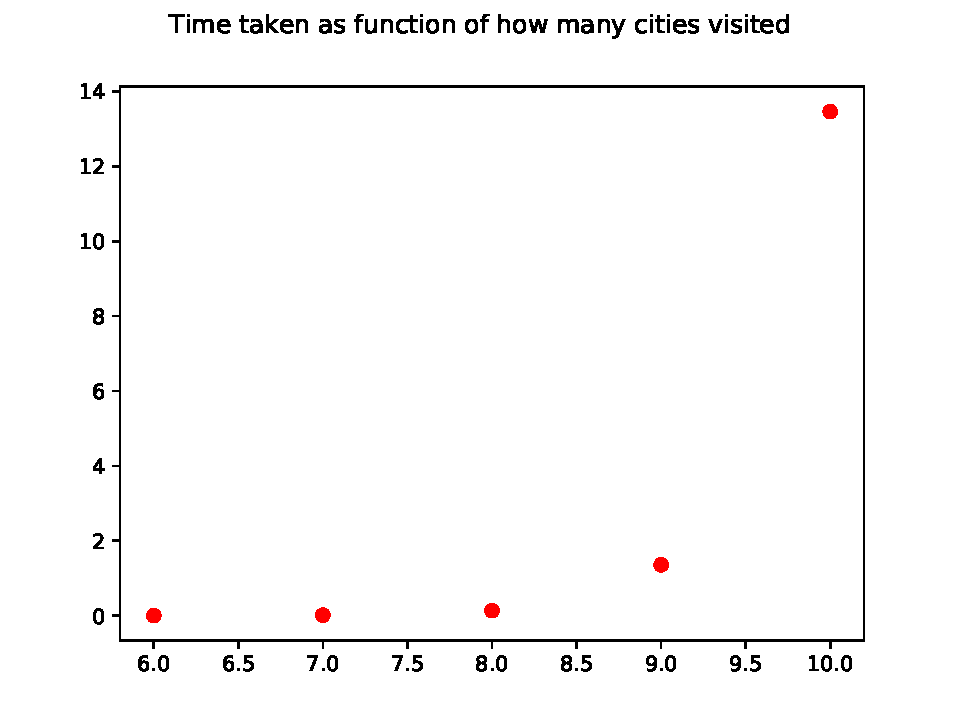
\includegraphics[scale=0.8]{"../Exhaustive.pdf}
\caption{Time spent for the TSP algorithm}
\end{center}
\end{figure}
\noindent
It can be seen that time spent by the algorithm searching for an optimal solution in TSP for  \textit{n} cities is roughly the time spent on searching for \textit{n-1} cities multiplied by \textit{n}. The time spent by the algorithm (on my laptop) to search for the optimal solution in TSP for 24 cities can be calculated with
\[
	t_{10} \frac{24!}{10!} \approx 14s \cdot \frac{24!}{10!} \approx 2.4 \cdot 10^{18}
\]
which is around 76 billion years.

\section{Hill Climbing}
This algorithm was made based on \cite[chapter 9.4.3]{marsland}. 
 
Start the program with
\begin{lstlisting}[language=bash]
	$ python3 hill_climber.py european_cities.csv 
\end{lstlisting}
The program will try to find the shortest route between 10 and the shortest route between 24 cities. The program outputs

\begin{lstlisting}[language=bash]
	For 10 cities:
	Running the algorithm 20 times
	Number of searches per round: 10000
	Best distance: 7503.099999999999
	Worst distance: 8324.82
	Average distance: 7835.56
	Standard deviation: 229.896
	Time taken per search[seconds]: 0.145487
 
	For 24 cities:
	Running the algorithm 20 times
	Number of searches per round: 10000
	Best distance: 19413.899999999998
	Worst distance: 22341.170000000006
	Average distance: 21236.6
	Standard deviation: 751.52
	Time taken per search[seconds]: 2.017303
\end{lstlisting}
\noindent
The best result of 20 hill climber runs gets close to the solution computed by the exhaustive search (7503 vs 7486). Results of 7486 have a been observed during test runs.

The hill climber uses 10000 iterations each run, using a total of 200000 iterations to find this result. The exhaustive search on the other hand uses 10! = 3628800 iterations.

Increasing the iterations used by the hill climber reduces the standard deviation and increases the chances of it finding the optimal distance.

When searching 24 cities, the hill climber uses around two seconds every run, resulting in a total of around 40 seconds for the whole run. This is in strong contrast to the 76 billion years of the exhaustive search. However, the result found is quite far from the optimal one, but gets better if number of iterations increases.

\section{Genetic algorithm}
This algorithm was made based on \cite[chapter 3 - 6]{eiben}. All in all, the algorithm consist of:
\begin{itemize}
\item An initializer: random permutations computed using numpy.
\item A parent selector: using a linear ranking scheme with \textit{s} = 1.5.
\item A crossover algorithm: cycle crossover.
\item A mutating scheme: inversion of subset of cities in the children. Probability of mutation: 50\%
\item Survivor selector: GENITOR. The \textit{n} weakest parents are replaced by \textit{n} children. I have chosen \textit{n} = 4 for all my runs.
\end{itemize}
\noindent
The program was tested with a population of 10, 50 and 100.

Start the program with
\begin{lstlisting}[language=bash]
	$ python3 genetic_algorithm.py european_cities.csv 
\end{lstlisting}
The program will try to find the shortest distance between 24 cities using the three different population sizes, and then do the same with 10 cities. The program outputs:
\begin{lstlisting}[language=bash]
	Search: 24 cities, population size: 10, number of generations: 500, 
	number of rounds: 20, number of children: 4: 
	Best distance: 12973.490000000002
	Worst distance: 17104.000000000004
	Average distance: 15060.7
	Standard deviation: 1068.48
	Time [seconds]: 3.821806
	Best order of travel: 
	Istanbul Bucharest Belgrade Kiev Moscow Saint Petersburg Stockholm Warsaw 			Berlin Copenhagen Hamburg Prague Vienna Budapest Milan Paris Madrid 				Barcelona Dublin London Brussels Munich Rome Istanbul
 
	Search: 24 cities, population size: 50, number of generations: 500, 
	number of rounds: 20, number of children: 4: 
	Best distance: 15061.940000000002
	Worst distance: 19732.84
	Average distance: 17479.9
	Standard deviation: 1168.88
	Time [seconds]: 7.734567
	Best order of travel: 
	Budapest Vienna Paris Dublin London Hamburg Bucharest Istanbul Sofia Warsaw 		Berlin Copenhagen Stockholm Saint Petersburg Moscow Kiev Belgrade Madrid 			Rome Barcelona Milan Prague Brussels Budapest
 
	Search: 24 cities, population size: 100, number of generations: 500, 
	number of rounds: 20, number of children: 4: 
	Best distance: 17702.68
	Worst distance: 20805.450000000004
	Average distance: 19217.2
	Standard deviation: 908.324
	Time [seconds]: 13.321729
	Best order of travel: 
	Brussels Paris Dublin Hamburg Stockholm Kiev Belgrade Munich Milan London 			Barcelona Madrid Rome Warsaw Vienna Prague Budapest Sofia Istanbul Bucharest 	Moscow Saint Petersburg Copenhagen Brussels
 
	Search: 10 cities, population size: 10, number of generations: 500, 
	number of rounds: 20, number of children: 4: 
	Best distance: 7486.309999999999
	Worst distance: 7503.1
	Average distance: 7490.51
	Standard deviation: 7.27028
	Time [seconds]: 2.237474
	Best order of travel: 
	Belgrade Istanbul Bucharest Budapest Berlin Copenhagen Hamburg Brussels 			Dublin Belgrade
 
	Search: 10 cities, population size: 50, number of generations: 500, 
	number of rounds: 20, number of children: 4: 
	Best distance: 7486.3099999999995
	Worst distance: 7503.1
	Average distance: 7490.51
	Standard deviation: 7.27028
	Time [seconds]: 4.680307
	Best order of travel: 
	Brussels Dublin Barcelona Belgrade Istanbul Bucharest Budapest Berlin 				Copenhagen Brussels
 
	Search: 10 cities, population size: 50, number of generations: 500, 
	number of rounds: 20, number of children: 4: 
	Best distance: 7486.3099999999995
	Worst distance: 7503.099999999999
	Average distance: 7487.15
	Standard deviation: 3.6593
	Time [seconds]: 4.920473
	Best order of travel: 
	Barcelona Belgrade Istanbul Bucharest Budapest Berlin Copenhagen Hamburg 			Brussels Barcelona
\end{lstlisting}
\noindent
A plot of the average fitness of the best individual of each generation can be seen in figure 2.
\begin{figure}[H]
\begin{center}
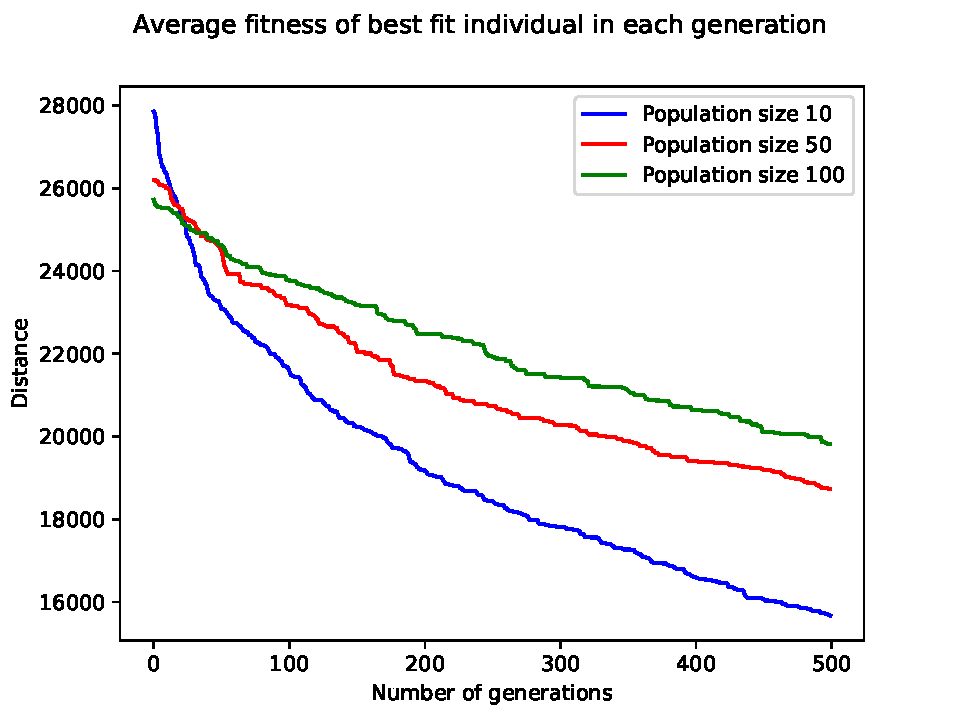
\includegraphics[scale=0.8]{"../genetic_algorithm.pdf}
\caption{Average fitness result for the genetic algorithm}
\end{center}
\end{figure}
As shown in the plot and the output, the algorithm converges slower as population size increases. A reason for this might be because the survivor selection do not scale with the population size (\textit{n} = 4 for all population sizes). For this setup, the smaller population size (or the bigger ratio between \textit{n} and population size) gives the most effective and fruitful search.



\section{Hybrid algorithm}
Use hill climber on each individual as part of the evaluation, report min max mean deviation and average fitness with both Lamarckian and Baldwinian learning models, Compare result with GA
\subsection{Lamarckian learning model}
\begin{lstlisting}[language=bash]
---- LAMARCKIAN LEARNING MODEL ----
Search: 24 cities, population size: 10, number of generations: 500, 
number of rounds: 20, number of children: 4,number of hill climb iterations: 3: 
Best distance: 12416.869999999999
Worst distance: 14093.089999999998
Average distance: 13252.1
Standard deviation: 450.395
Time [seconds]: 17.240872
Best order of travel: 
Bucharest Istanbul Sofia Belgrade Budapest Vienna Milan Rome Barcelona 
Madrid Paris Brussels Munich Prague Berlin Hamburg London Dublin Copenhagen 
Stockholm Saint Petersburg Moscow Kiev Bucharest
 
Search: 24 cities, population size: 50, number of generations: 500, 
number of rounds: 20, number of children: 4, number of hill climb iterations: 3: 
Best distance: 12325.93
Worst distance: 13547.129999999997
Average distance: 12939.1
Standard deviation: 331.192
Time [seconds]: 71.480543
Best order of travel: 
Dublin London Paris Brussels Hamburg Prague Vienna Budapest Belgrade Sofia 
Istanbul Bucharest Berlin Copenhagen Stockholm Saint Petersburg Moscow Kiev 
Warsaw Munich Milan Rome Barcelona Dublin
 
Search: 24 cities, population size: 100, number of generations: 500, 
number of rounds: 20, number of children: 4 number of hill climb iterations: 3: 
Best distance: 12520.170000000002
Worst distance: 13455.670000000002
Average distance: 12983.2
Standard deviation: 254.007
Time [seconds]: 140.06269
Best order of travel: 
Copenhagen Stockholm Saint Petersburg Moscow Kiev Warsaw Budapest Bucharest 
Istanbul Sofia Belgrade Vienna Munich Milan Rome Barcelona Madrid Dublin 
London Paris Brussels Prague Berlin Copenhagen
 
Search: 10 cities, population size: 10, number of generations: 500, 
number of rounds: 20, number of children: 4 number of hill climb iterations: 3: 
Best distance: 7486.309999999999
Worst distance: 7486.31
Average distance: 7486.31
Standard deviation: 5.85938e-05
Time [seconds]: 9.794478
Best order of travel: 
Istanbul Bucharest Budapest Berlin Copenhagen Hamburg Brussels Dublin Barcelona 
Istanbul
 
Search: 10 cities, population size: 50, number of generations: 500, 
number of rounds: 20, number of children: 4 number of hill climb iterations: 3: 
Best distance: 7486.309999999999
Worst distance: 7486.3099999999995
Average distance: 7486.31
Standard deviation: 5.85938e-05
Time [seconds]: 40.547498
Best order of travel: 
Brussels Dublin Barcelona Belgrade Istanbul Bucharest Budapest Berlin Copenhagen 
Brussels
 
Search: 10 cities, population size: 100, number of generations: 500, 
number of rounds: 20, number of children: 4 number of hill climb iterations: 3: 
Best distance: 7486.309999999999
Worst distance: 7486.3099999999995
Average distance: 7486.31
Standard deviation: 5.85938e-05
Time [seconds]: 79.250088
Best order of travel: 
Budapest Bucharest Istanbul Belgrade Barcelona Dublin Brussels Hamburg Copenhagen 
Budapest
\end{lstlisting}

\begin{figure}[H]
\begin{center}
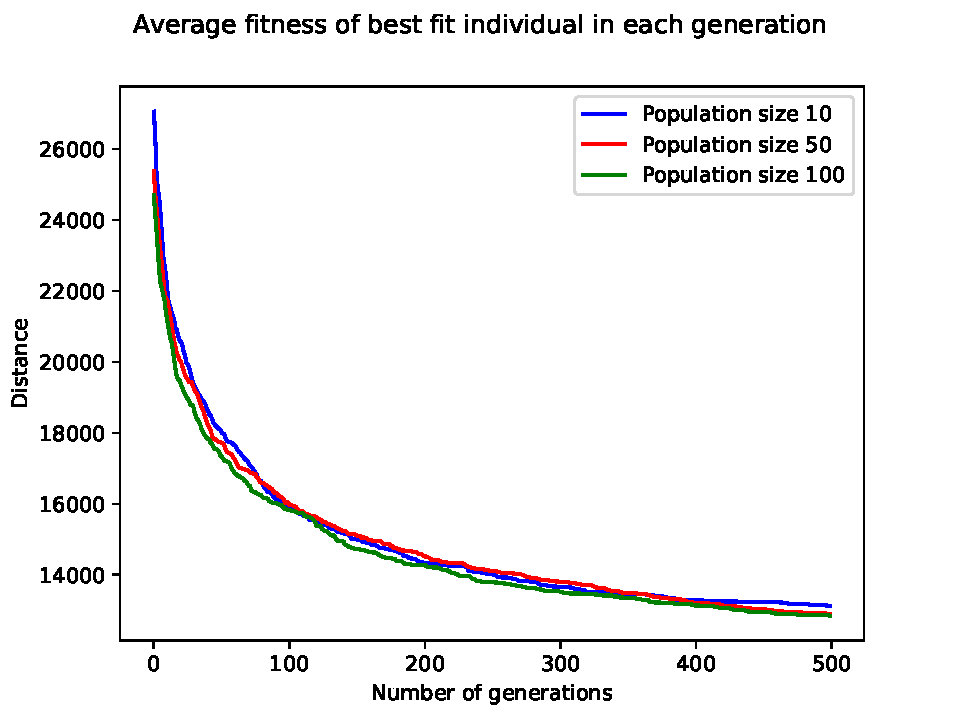
\includegraphics[scale=0.8]{"../hybrid_algorithm_lamarckian.pdf}
\caption{Average fitness result for the hybrid algorithm with a Lamarckian learning model}
\end{center}
\end{figure}

\subsection{Baldwinian learning model}
\begin{lstlisting}[language=bash]
---- BALDWINIAN LEARNING MODEL ----
Search: 24 cities, population size: 10, number of generations: 500, 
number of rounds: 20, number of children: 4 number of hill climb iterations: 3: 
Best distance: 23569.699999999997
Worst distance: 30698.32
Average distance: 27057.8
Standard deviation: 1698.52
Time [seconds]: 19.73016
Best order of travel: 
Paris Sofia Istanbul Bucharest Warsaw Dublin Berlin Belgrade Moscow Kiev Saint 
Petersburg Stockholm Vienna Milan Budapest London Brussels Copenhagen Madrid 
Rome Munich Barcelona Hamburg Paris
 
Search: 24 cities, population size: 50, number of generations: 500, 
number of rounds: 20, number of children: 4 number of hill climb iterations: 3: 
Best distance: 23313.62
Worst distance: 33411.56
Average distance: 27435.2
Standard deviation: 2288.74
Time [seconds]: 89.600072
Best order of travel: 
Vienna Belgrade Hamburg Copenhagen Stockholm Saint Petersburg Moscow Milan Kiev 
Berlin Prague Brussels Sofia Barcelona Warsaw London Dublin Paris Budapest 
Bucharest Istanbul Rome Madrid Vienna
 
Search: 24 cities, population size: 100, number of generations: 500, 
number of rounds: 20, number of children: 4 number of hill climb iterations: 3: 
Best distance: 24248.28
Worst distance: 31721.629999999994
Average distance: 27034.7
Standard deviation: 2062.25
Time [seconds]: 188.508705
Best order of travel: 
Hamburg Prague Saint Petersburg Moscow Belgrade Copenhagen Berlin Paris Brussels 
Milan Vienna Warsaw Rome Dublin London Stockholm Budapest Istanbul Kiev Barcelona 
Madrid Sofia Bucharest Hamburg
 
Search: 10 cities, population size: 10, number of generations: 500, 
number of rounds: 20, number of children: 4 number of hill climb iterations: 3: 
Best distance: 8612.61
Worst distance: 15709.300000000001
Average distance: 11665.6
Standard deviation: 2025.71
Time [seconds]: 14.102291
Best order of travel: 
Budapest Belgrade Istanbul Barcelona Hamburg Brussels Copenhagen Dublin Berlin 
Budapest
 
Search: 10 cities, population size: 50, number of generations: 500, 
number of rounds: 20, number of children: 4 number of hill climb iterations: 3: 
Best distance: 8312.79
Worst distance: 12810.14
Average distance: 10222.6
Standard deviation: 1503.26
Time [seconds]: 51.040574
Best order of travel: 
Belgrade Bucharest Dublin Copenhagen Berlin Budapest Hamburg Brussels Barcelona 
Belgrade
 
Search: 10 cities, population size: 100, number of generations: 500, 
number of rounds: 20, number of children: 4 number of hill climb iterations: 3: 
Best distance: 8450.56
Worst distance: 15331.689999999999
Average distance: 11454.8
Standard deviation: 1912.34
Time [seconds]: 99.088864
Best order of travel: 
Bucharest Copenhagen Hamburg Berlin Brussels Dublin Budapest Barcelona Belgrade 
Bucharest

\end{lstlisting}

\begin{figure}[H]
\begin{center}
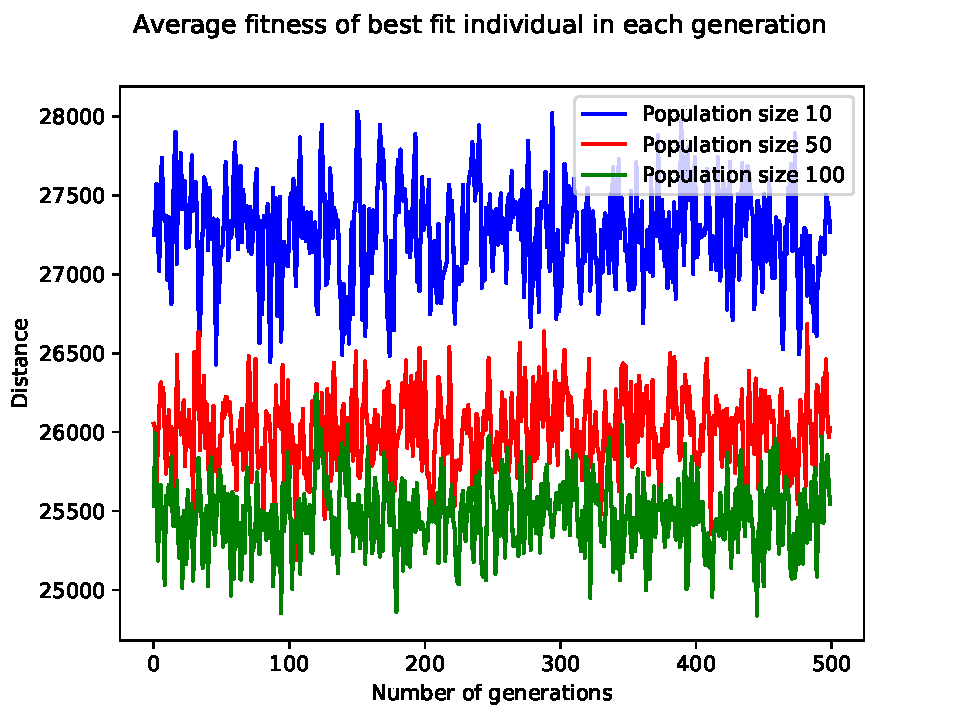
\includegraphics[scale=0.8]{"../hybrid_algorithm_baldwinian.pdf}
\caption{Average fitness result for the hybrid algorithm with a Baldwinian learning model}
\end{center}
\end{figure}

\begin{thebibliography}{9}

\bibitem{eiben}
  A.E Eiben, J.E Smith,
  \textit{Introduction to Evolutionary Computing},
  Springer, London,
  2nd edition,
  2015.
  
\bibitem{marsland}
  Stephen Marsland,
  \textit{Machine Learning - An Algorithmic Perspective},
  Chapman and Hall/CRC, Boca Raton/London/New York,
  2nd edition,
  2015.

\end{thebibliography}

\end{document}
